
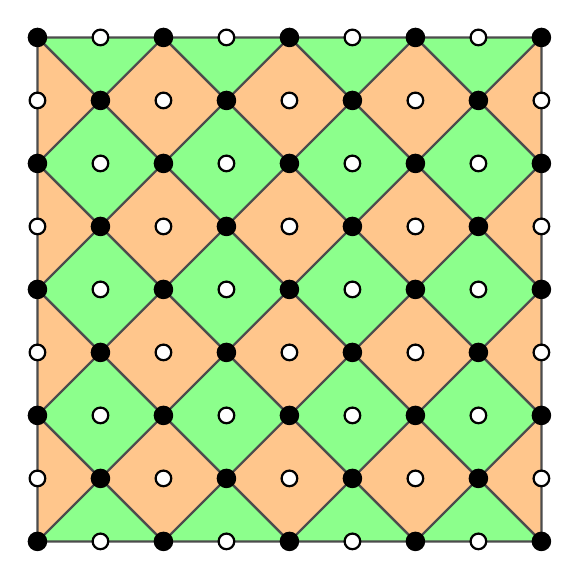
\begin{tikzpicture}[scale=0.8]
    \colorlet{zcolor}{green!45}  % Z stabilizers (Plaquettes)
    \colorlet{xcolor}{orange!45} % X stabilizers (Stars)

  
    \foreach \x in {1, 3, 5, 7} {
        \foreach \y in {0, 2, 4, 6, 8} {
            \ifnum\y=0
                % Bottom boundary Z stabilizers (Weight-3)
                \filldraw[fill=zcolor, draw=black!70, thick, rounded corners=2pt] 
                    (\x-1,0) -- (\x,1) -- (\x+1,0) -- cycle;
            \else\ifnum\y=8
                % Top boundary Z stabilizers (Weight-3)
                \filldraw[fill=zcolor, draw=black!70, thick, rounded corners=2pt] 
                    (\x-1,8) -- (\x,7) -- (\x+1,8) -- cycle;
            \else
                % Inner Z stabilizers (Weight-4)
                \filldraw[fill=zcolor, draw=black!70, thick, rounded corners=2pt] 
                    (\x-1,\y) -- (\x,\y+1) -- (\x+1,\y) -- (\x,\y-1) -- cycle;
            \fi\fi
        }
    }

    \foreach \x in {0, 2, 4, 6, 8} {
        \foreach \y in {1, 3, 5, 7} {
            \ifnum\x=0
                % Left boundary X stabilizers (Weight-3)
                \filldraw[fill=xcolor, draw=black!70, thick, rounded corners=2pt] 
                    (0,\y-1) -- (1,\y) -- (0,\y+1) -- cycle;
            \else\ifnum\x=8
                % Right boundary X stabilizers (Weight-3)
                \filldraw[fill=xcolor, draw=black!70, thick, rounded corners=2pt] 
                    (8,\y-1) -- (7,\y) -- (8,\y+1) -- cycle;
            \else
                % Inner X stabilizers (Weight-4)
                \filldraw[fill=xcolor, draw=black!70, thick, rounded corners=2pt] 
                    (\x-1,\y) -- (\x,\y+1) -- (\x+1,\y) -- (\x,\y-1) -- cycle;
            \fi\fi
        }
    }

   \foreach \x in {0, 2, 4, 6, 8} {
        \foreach \y in {0, 2, 4, 6, 8} {
            \node[circle, fill=black, inner sep=2.5pt] at (\x,\y) {};
        }
    }
    
    \foreach \x in {1, 3, 5, 7} {
        \foreach \y in {1, 3, 5, 7} {
            \node[circle, fill=black, inner sep=2.5pt] at (\x,\y) {};
        }
    }

   \foreach \x in {0, 2, 4, 6, 8} {
        \foreach \y in {1, 3, 5, 7} {
            \node[circle, fill=white, draw=black, thick, inner sep=2pt] at (\x,\y) {};
        }
    }
    
    \foreach \x in {1, 3, 5, 7} {
        \foreach \y in {0, 2, 4, 6, 8} {
            \node[circle, fill=white, draw=black, thick, inner sep=2pt] at (\x,\y) {};
        }
    }


\end{tikzpicture}
